\documentclass[11pt,a4paper]{report}
\usepackage[textwidth=37em,vmargin=30mm]{geometry}
\usepackage{calc,xunicode,amsmath,amssymb,paralist,enumitem,tabu,booktabs,datetime2,xeCJK,xeCJKfntef,listings}
\usepackage{tocloft,fancyhdr,tcolorbox,xcolor,graphicx,eso-pic,xltxtra,xelatexemoji}

\newcommand{\envyear}[0]{2025}
\newcommand{\envdatestr}[0]{2025-04-24}
\newcommand{\envfinaldir}[0]{webdb/2025/20250424/final}

\usepackage[hidelinks]{hyperref}
\hypersetup{
    colorlinks=false,
    pdfpagemode=FullScreen,
    pdftitle={Web Digest - \envdatestr}
}

\setlength{\cftbeforechapskip}{10pt}
\renewcommand{\cftchapfont}{\rmfamily\bfseries\large\raggedright}
\setlength{\cftbeforesecskip}{2pt}
\renewcommand{\cftsecfont}{\sffamily\small\raggedright}

\setdefaultleftmargin{2em}{2em}{1em}{1em}{1em}{1em}

\usepackage{xeCJK,xeCJKfntef}
\xeCJKsetup{PunctStyle=plain,RubberPunctSkip=false,CJKglue=\strut\hskip 0pt plus 0.1em minus 0.05em,CJKecglue=\strut\hskip 0.22em plus 0.2em}
\XeTeXlinebreaklocale "zh"
\XeTeXlinebreakskip = 0pt


\setmainfont{Brygada 1918}
\setromanfont{Brygada 1918}
\setsansfont{IBM Plex Sans}
\setmonofont{JetBrains Mono NL}
\setCJKmainfont{Noto Serif CJK SC}
\setCJKromanfont{Noto Serif CJK SC}
\setCJKsansfont{Noto Sans CJK SC}
\setCJKmonofont{Noto Sans CJK SC}

\setlength{\parindent}{0pt}
\setlength{\parskip}{8pt}
\linespread{1.15}

\lstset{
	basicstyle=\ttfamily\footnotesize,
	numbersep=5pt,
	backgroundcolor=\color{black!5},
	showspaces=false,
	showstringspaces=false,
	showtabs=false,
	tabsize=2,
	captionpos=b,
	breaklines=true,
	breakatwhitespace=true,
	breakautoindent=true,
	linewidth=\textwidth
}






\newcommand{\coverpic}[2]{
    % argv: itemurl, authorname
    Cover photo by #2~~(\href{#1}{#1})
}
\newcommand{\makeheader}[0]{
    \begin{titlepage}
        % \newgeometry{hmargin=15mm,tmargin=21mm,bmargin=12mm}
        \begin{center}
            
            \rmfamily\scshape
            \fontspec{BaskervilleF}
            \fontspec{Old Standard}
            \fontsize{59pt}{70pt}\selectfont
            WEB\hfill DIGEST
            
            \vfill
            % \vskip 30pt
            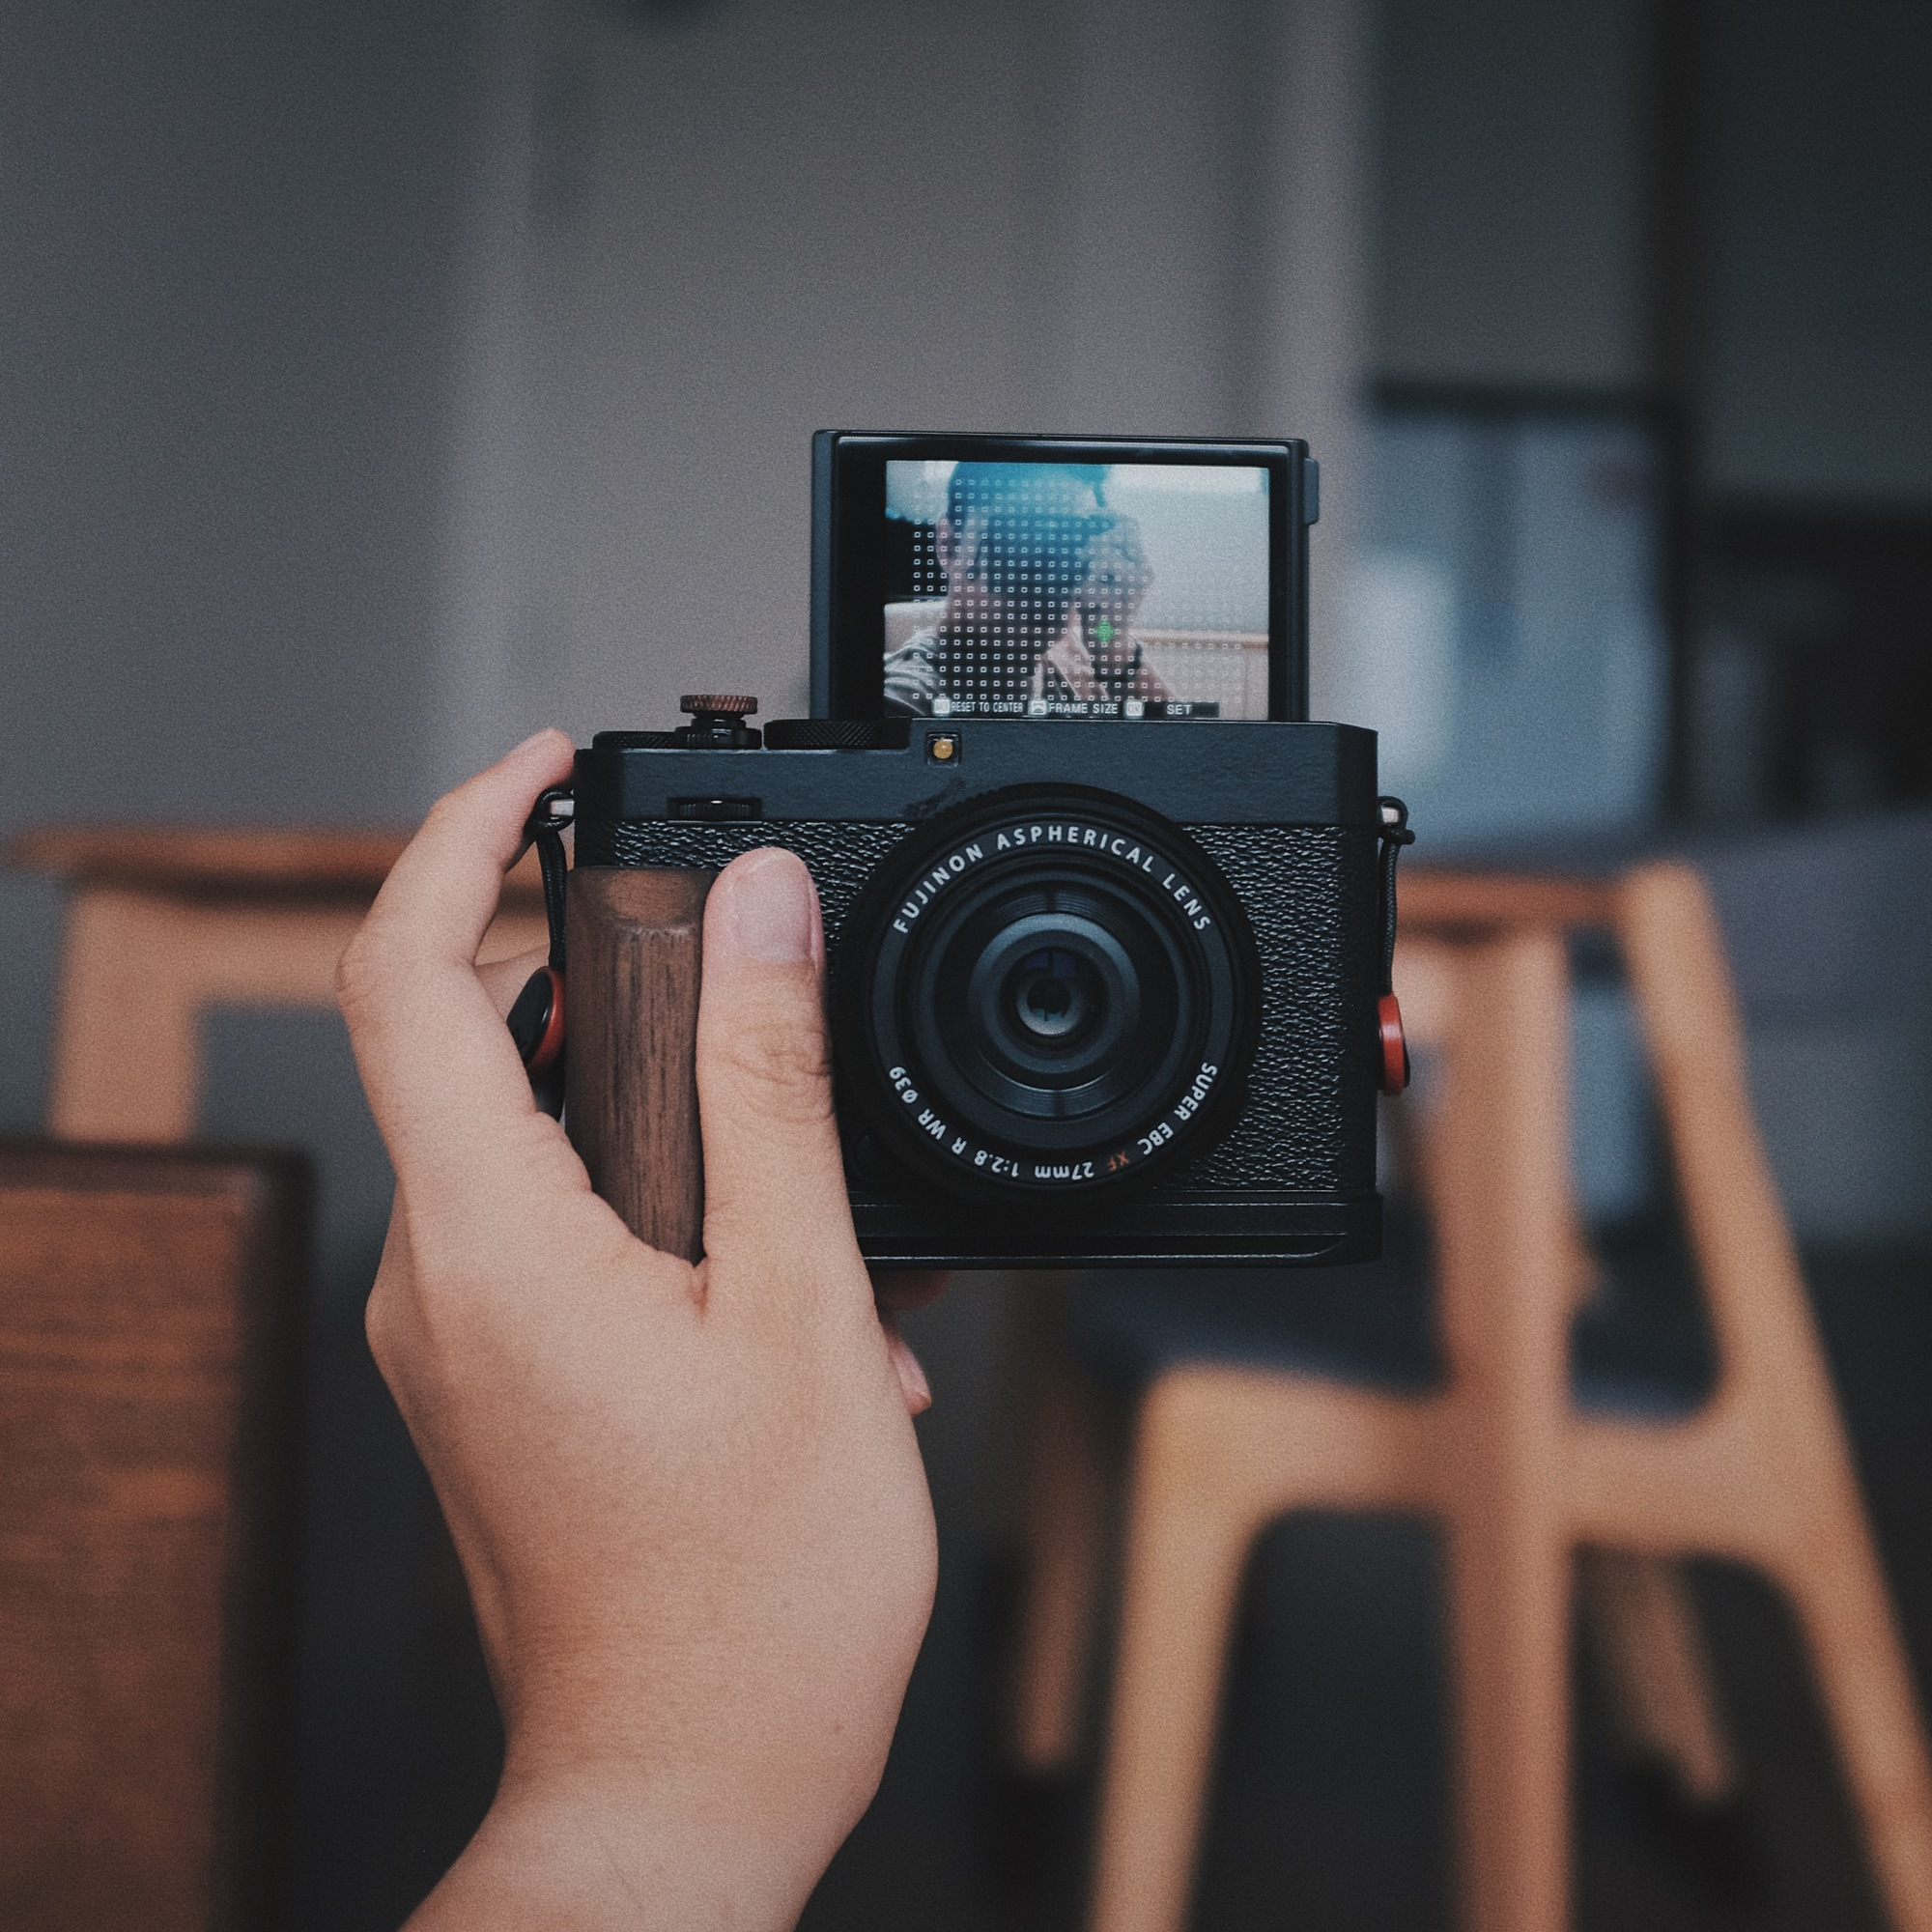
\includegraphics[width=\linewidth]{\envfinaldir/coverpic-prod.jpg}\par
            % \vskip 30pt
            \vfill

            \normalsize\rmfamily\scshape
            \copyright{} The Web Digest Project \hfill\large \envdatestr
        \end{center}
    \end{titlepage}
    % \restoregeometry
}
\newcommand{\simplehref}[1]{%
    \textcolor{blue!80!green}{\href{#1}{#1}}%
}
\renewcommand{\contentsname}{\center\Huge\sffamily\bfseries Contents\par\vskip 20pt}
\newcounter{ipartcounter}
\setcounter{ipartcounter}{0}
\newcommand{\ipart}[1]{
    % \vskip 20pt
    \clearpage
    \stepcounter{ipartcounter}
    \phantomsection
    \addcontentsline{toc}{chapter}{#1}
    % \begin{center}
    %     \Huge
    %     \sffamily\bfseries
    %     #1
    % \end{center}
    % \vskip 20pt plus 7pt
}
\newcounter{ichaptercounter}
\setcounter{ichaptercounter}{0}
\newcommand{\ichapter}[1]{
    % \vskip 20pt
    \clearpage
    \stepcounter{ichaptercounter}
    \phantomsection
    \addcontentsline{toc}{section}{\numberline{\arabic{ichaptercounter}}#1}
    \begin{center}
        \Huge
        \sffamily\bfseries
        #1
    \end{center}
    \vskip 20pt plus 7pt
}
\newcommand{\entrytitlefont}[1]{\subsection*{\raggedright\Large\sffamily\bfseries#1}}
\newcommand{\entryitemGeneric}[2]{
    % argv: title, url
    \parbox{\linewidth}{
        \entrytitlefont{#1}\par\vskip 5pt
        \footnotesize\ttfamily\mdseries
        \simplehref{#2}
    }\vskip 11pt plus 11pt minus 1pt
}
\newcommand{\entryitemGithub}[3]{
    % argv: title, url, desc
    \parbox{\linewidth}{
        \entrytitlefont{#1}\par\vskip 5pt
        \footnotesize\ttfamily\mdseries
        \simplehref{#2}\par\vskip 5pt
        \small\rmfamily\mdseries#3
    }\vskip 11pt plus 11pt minus 1pt
}
\newcommand{\entryitemAp}[3]{
    % argv: title, url, desc
    \parbox{\linewidth}{
        \entrytitlefont{#1}\par\vskip 5pt
        \footnotesize\ttfamily\mdseries
        \simplehref{#2}\par\vskip 5pt
        \small\rmfamily\mdseries#3
    }\vskip 11pt plus 11pt minus 1pt
}
\newcommand{\entryitemHackernews}[3]{
    % argv: title, hnurl, rawurl
    % \parbox{\linewidth}{
    %     \entrytitlefont{#1}\par\vskip 5pt
    %     \footnotesize\ttfamily\mdseries
    %     \simplehref{#3}\par
    %     \textcolor{black!50}{\href{#2}{#2}}
    % }\vskip 11pt plus 11pt minus 1pt
    \begin{minipage}{\linewidth}
            \entrytitlefont{#1}\par\vskip 5pt
            \footnotesize\ttfamily\mdseries
            \simplehref{#3}\par
            \textcolor{black!50}{\href{#2}{#2}}
    \end{minipage}\par\vskip 11pt plus 11pt minus 1pt
}







\begin{document}

\makeheader

\tableofcontents\clearpage




\ipart{Developers}
\ichapter{Hacker News}
\entryitemTwoLinks{DOGE Worker's Code Supports NLRB Whistleblower}{https://news.ycombinator.com/item?id=43776476}{https://krebsonsecurity.com/2025/04/doge-workers-code-supports-nlrb-whistleblower/}

\entryitemTwoLinks{You wouldn't steal a font}{https://news.ycombinator.com/item?id=43775926}{https://fedi.rib.gay/notes/a6xqityngfubsz0f}

\entryitemTwoLinks{Teaching LLMs how to solid model}{https://news.ycombinator.com/item?id=43774990}{https://willpatrick.xyz/technology/2025/04/23/teaching-llms-how-to-solid-model.html}

\entryitemTwoLinks{I won't be vibe coding anymore: a noob's perspective}{https://news.ycombinator.com/item?id=43773977}{https://varunraghu.com/why-i-wont-be-vibe-coding-anymore/}

\entryitemTwoLinks{AI Horseless Carriages}{https://news.ycombinator.com/item?id=43773813}{https://koomen.dev/essays/horseless-carriages/}

\entryitemTwoLinks{They made computers behave like annoying salesmen}{https://news.ycombinator.com/item?id=43773710}{https://rakhim.exotext.com/they-made-computers-behave-like-annoying-salesmen}

\entryitemTwoLinks{How a 20 year old bug in GTA San Andreas surfaced in Windows 11 24H2}{https://news.ycombinator.com/item?id=43772311}{https://cookieplmonster.github.io/2025/04/23/gta-san-andreas-win11-24h2-bug/}

\entryitemTwoLinks{How I blog with Obsidian, Hugo, GitHub, and Cloudflare}{https://news.ycombinator.com/item?id=43771645}{https://ingau.me/blog/how-i-write-my-blogs-in-obsidian-and-publish-instantly/}

\entryitemTwoLinks{Show HN: Node.js video tutorials where you can edit and run the code}{https://news.ycombinator.com/item?id=43771365}{https://news.ycombinator.com/item?id=43771365}

\entryitemTwoLinks{Geocoding APIs compared: Pricing, free tiers and terms of use}{https://news.ycombinator.com/item?id=43770446}{https://www.bitoff.org/geocoding-apis-comparison/}

\entryitemTwoLinks{MinC Is Not Cygwin}{https://news.ycombinator.com/item?id=43770445}{https://minc.commandlinerevolution.nl/english/home.html}

\entryitemTwoLinks{EU fines Apple €500M and Meta €200M}{https://news.ycombinator.com/item?id=43770396}{https://www.politico.eu/article/eu-fines-apple-meta-breaking-europe-digital-markets-act-dma/}

\entryitemTwoLinks{America's cyber defenses are being dismantled from the inside}{https://news.ycombinator.com/item?id=43770382}{https://www.theregister.com/2025/04/23/trump\_us\_security/}

\entryitemTwoLinks{Apple and Meta fined millions for breaching EU law}{https://news.ycombinator.com/item?id=43770337}{https://ca.finance.yahoo.com/news/apple-fined-570-million-meta-094701712.html}

\entryitemTwoLinks{OpenAI wants to buy Chrome and make it an "AI-first" experience}{https://news.ycombinator.com/item?id=43770312}{https://arstechnica.com/ai/2025/04/chatgpt-head-tells-court-openai-is-interested-in-buying-chrome/}

\entryitemTwoLinks{The Gruen Transfer is consuming the internet}{https://news.ycombinator.com/item?id=43769936}{https://sebs.website/blog/the\%20gruen-transfer-is-consuming-the-internet}

\entryitemTwoLinks{Advanced Python Features}{https://news.ycombinator.com/item?id=43769486}{https://blog.edward-li.com/tech/advanced-python-features/}

\entryitemTwoLinks{Open Source Projects Receive Funding to Reclaim the Public Internet}{https://news.ycombinator.com/item?id=43769482}{https://nlnet.nl/news/2025/20250422-announcement-grants-CommonsFund.html}

\entryitemTwoLinks{Pixel is a unit of length and area}{https://news.ycombinator.com/item?id=43769478}{https://www.nayuki.io/page/pixel-is-a-unit-of-length-and-area}

\entryitemTwoLinks{Native visionOS platform support}{https://news.ycombinator.com/item?id=43768421}{https://github.com/godotengine/godot/pull/105628}\ichapter{Phoronix}
\entryitemGeneric{\hskip 0pt{}OpenMandriva Lx 6.0 Brings KDE Plasma 6 By Default, Official Server Edition}{https://www.phoronix.com/news/OpenMandriva-Lx-6.0-Released}

\entryitemGeneric{\hskip 0pt{}Linux 6.15 Lands Fix For "3x Performance Regression" Affecting Nginx \& Other Software}{https://www.phoronix.com/review/linux-615-regression-fix}

\entryitemGeneric{\hskip 0pt{}Mesa 25.1-rc2 Released With NVK Vulkan 1.4 Conformance For Older NVIDIA GPUs}{https://www.phoronix.com/news/Mesa-25.1-rc2-Released}

\entryitemGeneric{\hskip 0pt{}Orange Pi RV2 Benchmarks: The Most Performant RISC-V Board For Less Than \$100 With 8 Cores + 8GB RAM}{https://www.phoronix.com/review/orange-pi-rv2-benchmarks}

\entryitemGeneric{\hskip 0pt{}AMD Posts Open-Source Linux Patches For Pensando RDMA Driver}{https://www.phoronix.com/news/AMD-Pensando-RDMA-Driver}

\entryitemGeneric{\hskip 0pt{}Ubuntu 25.10 Moving Ahead With Plans For Migrating To Rust Coreutils}{https://www.phoronix.com/news/Ubuntu-2510-Rust-Coreutils-Plan}

\entryitemGeneric{\hskip 0pt{}Fedora 43 Change Proposal Filed For Removing GNOME X11 Packages: Wayland-Only GNOME}{https://www.phoronix.com/news/F43-Change-Wayland-Only-GNOME}

\entryitemGeneric{\hskip 0pt{}VMware Updates Linux Patches For Running VMware Workstation Atop KVM}{https://www.phoronix.com/news/VMware-Workstation-Linux-KVM-v2}

\entryitemGeneric{\hskip 0pt{}Patches Hoping For The Upstream Kernel Finally Provide Google Pixel 4a Support}{https://www.phoronix.com/news/Google-Pixel-4a-Patches-Linux}\ichapter{GitHub}
\entryitemWithDescription{\hskip 0pt{}pocketbase/pocketbase}{https://github.com/pocketbase/pocketbase}{Open Source realtime backend in 1 file\\
Language: Go\\
Stars: 46129\\
Forks: 2265}\ichapter{Dribbble}
\entryitemGeneric{\hskip 0pt{}Travel Startup Branding for Holidu: visual identity brand design}{https://dribbble.com/shots/25916676-Travel-Startup-Branding-for-Holidu-visual-identity-brand-design}

\entryitemGeneric{\hskip 0pt{}Betpanda}{https://dribbble.com/shots/25937317-Betpanda}

\entryitemGeneric{\hskip 0pt{}Crypto Portfolio Tracker App}{https://dribbble.com/shots/25936470-Crypto-Portfolio-Tracker-App}

\entryitemGeneric{\hskip 0pt{}Unused Netomi Logo Concept}{https://dribbble.com/shots/25937558-Unused-Netomi-Logo-Concept}

\entryitemGeneric{\hskip 0pt{}Bismuth}{https://dribbble.com/shots/25933886-Bismuth}

\entryitemGeneric{\hskip 0pt{}boundless}{https://dribbble.com/shots/25930426-boundless}

\entryitemGeneric{\hskip 0pt{}Logo Design for Premium Online Store}{https://dribbble.com/shots/25931384-Logo-Design-for-Premium-Online-Store}

\entryitemGeneric{\hskip 0pt{}Tempora Logo Design - Hourglass, Time, Sand Clock}{https://dribbble.com/shots/25926528-Tempora-Logo-Design-Hourglass-Time-Sand-Clock}

\entryitemGeneric{\hskip 0pt{}OltreFluire}{https://dribbble.com/shots/25914855-OltreFluire}

\entryitemGeneric{\hskip 0pt{}Cruising for the coast}{https://dribbble.com/shots/25914452-Cruising-for-the-coast}

\entryitemGeneric{\hskip 0pt{}Tanuki - Raccoon, Animal Logo Design}{https://dribbble.com/shots/25917338-Tanuki-Raccoon-Animal-Logo-Design}

\entryitemGeneric{\hskip 0pt{}Bismuth}{https://dribbble.com/shots/25918310-Bismuth}

\entryitemGeneric{\hskip 0pt{}Logo Design for AI Companies}{https://dribbble.com/shots/25917078-Logo-Design-for-AI-Companies}

\entryitemGeneric{\hskip 0pt{}American Home Shield}{https://dribbble.com/shots/25916194-American-Home-Shield}

\entryitemGeneric{\hskip 0pt{}Case study: Educational Website on Space Pollution}{https://dribbble.com/shots/25914349-Case-study-Educational-Website-on-Space-Pollution}

\entryitemGeneric{\hskip 0pt{}Columbus Rapids®}{https://dribbble.com/shots/25915181-Columbus-Rapids}

\entryitemGeneric{\hskip 0pt{}Cute Easter Bunny Mascot}{https://dribbble.com/shots/25914543-Cute-Easter-Bunny-Mascot}

\entryitemGeneric{\hskip 0pt{}BB}{https://dribbble.com/shots/25913015-BB}

\entryitemGeneric{\hskip 0pt{}Phantom concept with Widget}{https://dribbble.com/shots/25911511-Phantom-concept-with-Widget}

\entryitemGeneric{\hskip 0pt{}Crypto Widget}{https://dribbble.com/shots/25913330-Crypto-Widget}

\entryitemGeneric{\hskip 0pt{}UNIC // Mobile App}{https://dribbble.com/shots/25913185-UNIC-Mobile-App}

\entryitemGeneric{\hskip 0pt{}Finance Platform website design}{https://dribbble.com/shots/25911576-Finance-Platform-website-design}

\entryitemGeneric{\hskip 0pt{}Finta}{https://dribbble.com/shots/25913820-Finta}

\entryitemGeneric{\hskip 0pt{}Towards the Cloud - Logo Redesign}{https://dribbble.com/shots/25914936-Towards-the-Cloud-Logo-Redesign}


\ipart{Developers~~~~(zh-Hans)}
\ichapter{Solidot}
\entryitemGeneric{\hskip 0pt{}昆虫在全世界以惊人的速度消失}{https://www.solidot.org/story?sid=81127}

\entryitemGeneric{\hskip 0pt{}脉冲星揭示星际等离子体结构}{https://www.solidot.org/story?sid=81126}

\entryitemGeneric{\hskip 0pt{}Google Chrome 将继续使用第三方 Cookies }{https://www.solidot.org/story?sid=81125}

\entryitemGeneric{\hskip 0pt{}英特尔计划裁掉逾五分之一员工}{https://www.solidot.org/story?sid=81124}

\entryitemGeneric{\hskip 0pt{}OpenAI 有意收购 Chrome}{https://www.solidot.org/story?sid=81123}

\entryitemGeneric{\hskip 0pt{}Bethesda 发布《上古卷轴IV:湮灭重制版》}{https://www.solidot.org/story?sid=81122}

\entryitemGeneric{\hskip 0pt{}OpenAI要30亿美金买的公司,Windsurf创始人Varun:创业无需每门功课是A,但不分部门,每个员工都要会用AI写代码}{https://www.solidot.org/story?sid=81121}

\entryitemGeneric{\hskip 0pt{}为什么说终身学习是AGI的最终形态?}{https://www.solidot.org/story?sid=81120}

\entryitemGeneric{\hskip 0pt{}华为准备大量供应升腾910C}{https://www.solidot.org/story?sid=81119}

\entryitemGeneric{\hskip 0pt{}野生黑猩猩会分享含酒精食物}{https://www.solidot.org/story?sid=81118}

\entryitemGeneric{\hskip 0pt{}单剂量致幻剂能在数周内提升大脑灵活性}{https://www.solidot.org/story?sid=81117}

\entryitemGeneric{\hskip 0pt{}全球酒精消费已过峰值}{https://www.solidot.org/story?sid=81116}

\entryitemGeneric{\hskip 0pt{}天文学家证实流浪黑洞的存在}{https://www.solidot.org/story?sid=81115}

\entryitemGeneric{\hskip 0pt{}宁德时代称其电池充电五分钟可行驶 520 公里}{https://www.solidot.org/story?sid=81112}

\entryitemGeneric{\hskip 0pt{}Python 3.14 将支持模板字符串}{https://www.solidot.org/story?sid=81111}

\entryitemGeneric{\hskip 0pt{}黄金期货突破每盎司 3500 美元}{https://www.solidot.org/story?sid=81110}

\entryitemGeneric{\hskip 0pt{}18 岁程序员停止开源应用 Whisky 开发,称担心伤害 CodeWeavers 的付费产品}{https://www.solidot.org/story?sid=81109}

\entryitemGeneric{\hskip 0pt{}欧盟表示不管企业位于何处都会执行数字市场法}{https://www.solidot.org/story?sid=81108}

\entryitemGeneric{\hskip 0pt{}地球上的水可能来自自身而不是小行星}{https://www.solidot.org/story?sid=81107}

\entryitemGeneric{\hskip 0pt{}异性恋女性部分依靠气味挑选朋友}{https://www.solidot.org/story?sid=81106}\ichapter{V2EX}
\entryitemGeneric{\hskip 0pt{}[NAS] 你的 NAS 上有部署开源的导航网站吗?}{https://www.v2ex.com/t/1127669}

\entryitemGeneric{\hskip 0pt{}[推广] 个人开发者如何发送短信?这个方案太香了!}{https://www.v2ex.com/t/1127668}

\entryitemGeneric{\hskip 0pt{}[程序员] 使用 dokploy 磁盘空间占用很多是什么原因呢?如何解决?}{https://www.v2ex.com/t/1127666}

\entryitemGeneric{\hskip 0pt{}[Go 编程语言] 我有一个日期时间的字段它有可能为空,我问 Go 该怎么办……}{https://www.v2ex.com/t/1127665}

\entryitemGeneric{\hskip 0pt{}[设计] 88x31 badges by Louie Mantia}{https://www.v2ex.com/t/1127664}

\entryitemGeneric{\hskip 0pt{}[电影] 恐怖片看多了,后劲很大。}{https://www.v2ex.com/t/1127663}

\entryitemGeneric{\hskip 0pt{}[PHP] workman 与阿里云实时语音通信的问题。}{https://www.v2ex.com/t/1127661}

\entryitemGeneric{\hskip 0pt{}[剧集] 行尸走肉是不是烂尾了啊?}{https://www.v2ex.com/t/1127660}

\entryitemGeneric{\hskip 0pt{}[Apple] mac 在直营店用 ac+换完电池之后,续航还是一般}{https://www.v2ex.com/t/1127659}

\entryitemGeneric{\hskip 0pt{}[Apple] 为什么 MacOS 不内置一个类似 Bartender 的功能?}{https://www.v2ex.com/t/1127658}

\entryitemGeneric{\hskip 0pt{}[分享创造] [网站自荐] Search Suggest Pro - 一站式搜索建议聚合平台,获取 9 大平台搜索建议,高效关键词研究工具}{https://www.v2ex.com/t/1127656}

\entryitemGeneric{\hskip 0pt{}[求职] 9 年 Java / Python 架构+后端,对工作机会开放,广州或者 remote}{https://www.v2ex.com/t/1127653}

\entryitemGeneric{\hskip 0pt{}[问与答] 发现个有意思的小程序 能解决吃什么的烦恼}{https://www.v2ex.com/t/1127652}

\entryitemGeneric{\hskip 0pt{}[宽带症候群] 深圳联通关于上行流量限制的通知}{https://www.v2ex.com/t/1127651}

\entryitemGeneric{\hskip 0pt{}[问与答] 一个以乐器为核心的交流论坛是否有搞头?}{https://www.v2ex.com/t/1127650}

\entryitemGeneric{\hskip 0pt{}[分享发现] 体会了到了什么叫做工具人}{https://www.v2ex.com/t/1127649}

\entryitemGeneric{\hskip 0pt{}[Go 编程语言] 调研一下,目前 Go 岗位的市场如何}{https://www.v2ex.com/t/1127648}

\entryitemGeneric{\hskip 0pt{}[SONY] 索尼手机工作应用 shizuku 权限没了}{https://www.v2ex.com/t/1127647}

\entryitemGeneric{\hskip 0pt{}[分享创造] 写了个玩具项目: LLM 对比测试平台,同时对比如 OpenAI、DeepSeek、Gemini 等平台 LLM 回答质量、响应速度}{https://www.v2ex.com/t/1127646}

\entryitemGeneric{\hskip 0pt{}[酷工作] 外企招聘,福利好,待遇优,急缺 ai 人才}{https://www.v2ex.com/t/1127645}

\entryitemGeneric{\hskip 0pt{}[Android] 分享一个自己开发的开源安卓 GPT 助手软件: GPT Assistant}{https://www.v2ex.com/t/1127644}

\entryitemGeneric{\hskip 0pt{}[问与答] 哪家第三方的 AI 提供商支持画图和视频生成的?}{https://www.v2ex.com/t/1127643}

\entryitemGeneric{\hskip 0pt{}[问与答] 有没有 UI 类似扣子的开源工作流引擎?}{https://www.v2ex.com/t/1127642}

\entryitemGeneric{\hskip 0pt{}[问与答] 阿里云 ecs Linux 想扩充一下硬盘,看文档操作步骤好繁琐,不敢动,有啥保险的办法吗?}{https://www.v2ex.com/t/1127640}

\entryitemGeneric{\hskip 0pt{}[Node.js] Cherry Studio 只用 bun.exe 怎么绕过去?}{https://www.v2ex.com/t/1127639}

\entryitemGeneric{\hskip 0pt{}[酷工作] [全职]广州 - 元图互动 - iOS 高级工程师}{https://www.v2ex.com/t/1127638}

\entryitemGeneric{\hskip 0pt{}[奇思妙想] 独立开发是否要遵守黑暗森林法则?}{https://www.v2ex.com/t/1127637}

\entryitemGeneric{\hskip 0pt{}[VXNA] 申请收录个人博客: 逻辑拾光}{https://www.v2ex.com/t/1127635}

\entryitemGeneric{\hskip 0pt{}[随想] 感觉大部分人有点毛病,但又不知道是哪里的毛病}{https://www.v2ex.com/t/1127634}

\entryitemGeneric{\hskip 0pt{}[MacBook Pro] 二手 99 新 14 寸 MacbookPro M4Pro(14+20) 48+512 纳米玻璃 15700 算好价吗?}{https://www.v2ex.com/t/1127633}

\entryitemGeneric{\hskip 0pt{}[问与答] 手机坏了,头一次感觉这么的孤独无助}{https://www.v2ex.com/t/1127632}

\entryitemGeneric{\hskip 0pt{}[问与答] apple tv 接电视,每次切换画面都黑屏是什么情况?}{https://www.v2ex.com/t/1127631}

\entryitemGeneric{\hskip 0pt{}[支付宝] 支付宝有没有能自动转账或者扣款的服务或者小程序?}{https://www.v2ex.com/t/1127630}

\entryitemGeneric{\hskip 0pt{}[问与答] RAG 召回率低?可能是知识库分段没做好!求问大佬们的经验​}{https://www.v2ex.com/t/1127629}

\entryitemGeneric{\hskip 0pt{}[汽车] 花了 2.7 万落地了微型车-奔腾小马}{https://www.v2ex.com/t/1127628}

\entryitemGeneric{\hskip 0pt{}[Apple] 收 2021 款 14 寸 MacBook Pro 16 + 512}{https://www.v2ex.com/t/1127625}

\entryitemGeneric{\hskip 0pt{}[问与答] vscode 有比较好的支持 markdown 的插件吗}{https://www.v2ex.com/t/1127624}

\entryitemGeneric{\hskip 0pt{}[Go 编程语言] 求一款稳定靠谱的分布式整型 ID 生成组件}{https://www.v2ex.com/t/1127623}

\entryitemGeneric{\hskip 0pt{}[分享创造] [应用更新] wedock 搜索插件-修复微信输入中文途中自动隐藏问题}{https://www.v2ex.com/t/1127622}

\entryitemGeneric{\hskip 0pt{}[问与答] 2025 年了,你们都用哪款外接键盘?}{https://www.v2ex.com/t/1127621}

\entryitemGeneric{\hskip 0pt{}[问与答] 预算一千以内,滚轮好的鼠标选什么?}{https://www.v2ex.com/t/1127620}

\entryitemGeneric{\hskip 0pt{}[程序员] 用 cursor 编程好像真的会让编程能力变弱}{https://www.v2ex.com/t/1127619}

\entryitemGeneric{\hskip 0pt{}[问与答] 3000 以下安卓还是 iPhone 15}{https://www.v2ex.com/t/1127617}

\entryitemGeneric{\hskip 0pt{}[问与答] UTools 这个产品大家用的多吗?我在想如果做一个服务器版本的 虚拟桌面 + UTools 是否可行?}{https://www.v2ex.com/t/1127616}

\entryitemGeneric{\hskip 0pt{}[生活] 男士买裤子,有什么推荐的吗}{https://www.v2ex.com/t/1127614}

\entryitemGeneric{\hskip 0pt{}[酷工作] [深圳] 嵌入式 Linux 底层软件工程师招聘}{https://www.v2ex.com/t/1127613}

\entryitemGeneric{\hskip 0pt{}[职场话题] 近期面试记录,没学历真是难顶}{https://www.v2ex.com/t/1127612}

\entryitemGeneric{\hskip 0pt{}[宽带症候群] 有没有干过 olt pon 设备的大哥解答一下?}{https://www.v2ex.com/t/1127610}

\entryitemGeneric{\hskip 0pt{}[Apple] iPhone 总是自动加入已忽略的 wifi}{https://www.v2ex.com/t/1127609}

\entryitemGeneric{\hskip 0pt{}[程序员] 后端 CRUD 不是逻辑更简单,为什么 AI 编程更擅长前端?我给 cursor 详细描述的业务逻辑它老是理解错,前端不详细讲倒是能有点样子}{https://www.v2ex.com/t/1127608}


\ipart{Generic News}
\ichapter{联合早报}
\entryitemWithDescription{沈泽玮:魔幻山城的中国式现代化演绎}{https://www.zaobao.com/news/china/story20250424-6234868}{时隔12年因工作再访重庆,春夏交替之际迎来烈日当空,与当年冬季旅游行走于山城迷雾的印象截然不同。 5000架无人机灯光秀,既展现科技力量也打造视觉盛宴;科企创始人讲述营商环境不断优化;村委会主任手捧涪陵榨菜分享东方酱腌菜``走出去''成果;火车司机传递通关速度如何带动互联互通跨境贸易;公安局交巡警总队科研处综合科科长讲述数字化赋能超大城市治理;社区党委书记分享中国特色``民主村''的前身今世……}

\entryitemWithDescription{中国网购平台将全面取消``仅退款''}{https://www.zaobao.com/news/china/story20250423-6234242}{在中国官方整治``内卷式竞争''的背景下,中国电商平台将全面取消``仅退款''选项。受访学者认为,此举有助行业回归良性竞争,是对电商市场的一次纠偏。 据《北京商报》报道,拼多多、淘宝、抖音、快手、京东等多个中国电商平台,星期二(4月22日)修改有关``仅退款''的相关条款,消费者申请``退款不退货'',将由商家自主处理……}

\entryitemWithDescription{3月人民币跨境收付占比刷新历史纪录}{https://www.zaobao.com/news/china/story20250423-6233857}{(华盛顿彭博电)随着美元的全球吸引力减弱、中美贸易紧张局势上升,3月中国投资者和贸易公司在国际结算中对人民币的使用大幅增加,创下历史纪录。 彭博社基于中国国家外汇管理局星期二(4月22日)公布的数据计算,3月中国大陆境内个人和机构的跨境业务中,人民币使用占比达 54.3\%,总额7249亿美元(9502亿新元)……}

\entryitemWithDescription{中国首次选拔训练外国航天员 巴基斯坦载荷专家有望进中国空间站短期工作}{https://www.zaobao.com/news/china/story20250423-6233118}{(北京综合讯)中国和巴基斯坦正在巴国开展航天员选拔工作,未来几年内将有一名巴基斯坦航天员有机会进入中国空间站执行短期飞行任务。 综合新华社与《中国航天报》消息,中国载人航天工程新闻发言人林西强星期三(23日)宣布,中巴正在巴基斯坦开展航天员的选拔工作,先在巴基斯坦进行初选,然后在中国进行复选和定选,将选拔两名巴基斯坦航天员到中国参加训练……}

\entryitemWithDescription{李家超:上任三年仅休两天假 为港付出``值得''}{https://www.zaobao.com/news/china/story20250423-6234174}{香港特首李家超近日透露,自己上任即将三年,至今只放过两天假,但他认为担任此职是使命,应把所有时间都投入工作,每当看到市民脸上有笑容,他就觉得一切的付出都``值得''。 李家超平日对个人生活极为低调,他星期二(4月22日)接受香港``now''电视台专访时罕有地谈及个人生活,忆述上任至今只试过两天完整休假,一天用来配眼镜,另一天是陪伴家人到医院……}

\entryitemWithDescription{中国多省公布首季GDP:浙江高技术产业增长快 广东低于全国平均水平}{https://www.zaobao.com/news/china/story20250423-6233417}{(杭州/广州综合讯)中国多个省市陆续公布今年一季度经济数据,坐拥``杭州六小龙''等科创企业的浙江地区生产总值(GDP)同比增长6\%,而传统外贸大省广东同比增长4.1\%,低于全国5.4\%的增幅。 浙江省星期一(4月21日)公布一季度GDP为2万2300亿元(人民币,下同,约4000亿新元),同比增长6%,增幅高于浙江年初设定的5.5\%左右的全年增长目标……}

\entryitemWithDescription{赖清德委任前副总统陈建仁 代表台湾出席教宗方济各丧礼}{https://www.zaobao.com/news/china/story20250423-6232538}{(台北综合讯)台湾外交部与梵蒂冈全力交涉,希望促成台湾总统赖清德参加已故教宗方济各的丧礼弥撒。但在双方会商后,改由台湾前副总统陈建仁代表出席。 台湾外交部星期三(4月23日)在官网发表声明称,经过台梵双方讨论,由于陈健仁曾六度晋见教宗方济各,并获教宗亲自颁授教廷宗座科学院院士证章,与教宗关系深厚,决定由陈建仁担任总统特使,代表台湾出席教宗丧礼……}

\entryitemWithDescription{中国限制韩企向美国国防承包商出口含重稀土产品}{https://www.zaobao.com/news/china/story20250423-6232023}{(伦敦 / 首尔综合讯)中国政府告诫韩国企业不要向美国国防承包商出口含有重稀土矿物的产品,违者可能会受其制裁。这项出口管制或将冲击高度依赖出口的韩国经济。 《韩国经济日报》引述当地生产电力变压器的企业消息人士称,目前已有至少两家生产商接获上述通知。其他收到通知的企业包括生产电池、显示器、电动汽车、航空航天和医疗设备的企业,这些产品都都以稀土为关键原料……}

\entryitemWithDescription{中国扩大试点范围 推动服务业开放提速}{https://www.zaobao.com/news/china/story20250423-6228260}{在中美贸易战升级引发全球不安的背景下,中国政府宣布加快推进服务业扩大开放试点,新增九个试点城市与155项试点任务,并突出对接高标准国际经贸规则。 受访学者认为,中国此举履行了继续推动全球化的承诺,有利于树立与美国贸易保护主义不同的形象,参与相关国际规则制定,并吸引更多外资进入其服务业……}

\entryitemWithDescription{台湾蓝白两党将携手上凯道向赖清德发出怒吼}{https://www.zaobao.com/news/china/story20250422-6228009}{台湾在野的国民党(蓝)主席朱立伦与民众党(白)主席黄国昌,星期二(4月22日)举行在野领袖峰会,双方都认为要抑制总统赖清德的专制独裁,但对于如何``倒赖''尚无具体共识。 朱立伦号召群众星期六(4月26日)到总统府前的凯达格兰大道``战独裁'',也邀黄国昌与会。黄国昌当面应允,称将代表民众党参加这场人民的主场,也期盼民众一起站出来向赖清德发出怒吼……}

\entryitemWithDescription{宁德时代推出钠离子电池品牌 或挑战锂电池的主导地位}{https://www.zaobao.com/news/china/story20250422-6226805}{(上海/北京综合讯)中国电池巨头宁德时代推出首个钠离子电池品牌``钠新'',该公司预计,在安全性、宽温性、能源可控性等方面具备优势的钠离子电池,未来将取代磷酸铁锂电池一半的市场……}

\entryitemWithDescription{台湾研究报告:中国大陆对台加大经贸魅力攻势}{https://www.zaobao.com/news/china/story20250422-6225886}{(台北路透电)中国大陆加大对台湾军事施压的同时,也在经贸上展开魅力攻势。一项研究显示,2024年有近四万名台湾人参加了大陆官方支持的会议和贸易展等商业活动。 据路透社报道,总部设在台湾的非政府组织``台湾资讯环境研究中心''(IORG)星期二(4月22日)公布的研究报告显示,2024年约有3万9374名台湾人参加了由大陆各级政府单位支持或主办的逾400场商业活动……}

\entryitemWithDescription{【东谈西论】黄仁勋会把中国市场拱手让给华为吗?}{https://www.zaobao.com/news/china/story20250422-6225863}{美国特朗普政府对英伟达``特供''中国的H20晶片祭出出口管制后,英伟达首席执行官黄仁勋旋风式访华,与中国总理何立峰、中国国际贸易促进委员会会长任鸿斌、上海市长龚正等会面,强调英伟达坚定不移服务中国市场的立场。 黄仁勋指出,中国市场对英伟达非常重要,中国产业的科技实力让人印象深刻,过去30年里让英伟达获益。 据英伟达估计,特朗普政府的禁令将给英伟达带来55亿美元的损失……}

\entryitemWithDescription{北京警告各国跟美谈判勿损中国利益}{https://www.zaobao.com/news/china/story20250421-6222233}{在中美关税战陷入僵局之际,中国官方首次向正与美国进行贸易谈判的第三方国家发出明确警告,呼吁这些国家不要与美国达成损害中国利益的协议,并形容这是``与虎谋皮'',最终只会``两头落空,损人不利己''。 受访学者指出,美国就对等关税与他国采取一对一谈判方式有欠公平,中国在道义上更占优势。不过,学者认为,中美在关税战中谁都未占上风,双方也尚未就谈判方式释放明确信号……}

\entryitemWithDescription{中印尼外长防长2+2对话机制 首次举行部长级会议}{https://www.zaobao.com/news/china/story20250421-6222640}{在美国对全球发起关税战的阴影下,中国与印度尼西亚外长防长对话机制下的首次部长级会议,星期一在北京举行,标志这项机制步入常态化。 据中国外交部网站消息,中国外交部长王毅与印尼外交部长苏吉奥诺、中国国防部长董军与印尼国防部长沙夫里,星期一(4月21日)共同主持两国外长防长``2+2''对话机制首次会议,并向媒体介绍了双方达成的共识……}

\entryitemWithDescription{台湾蓝白两党举行在野峰会讨论时局}{https://www.zaobao.com/news/china/story20250421-6222445}{台湾两大在野党将举行领袖峰会,讨论关税变局、司法正义、民主等议题,民众党主席黄国昌呼吁总统赖清德一同与会,团结台湾社会,莫再对立冲突。 国民党主席朱立伦与黄国昌将在星期二(4月22日)上午举行``把民主还给台湾:在野领袖峰会'',聚焦``美国高关税对台湾之冲击''、``司法正义与民主之捍卫''等议题,共商解决之道,意在向执政党释出蓝白站在同一阵线的信号……}

\entryitemWithDescription{中远海运批美港口费新规冲击全球航运业}{https://www.zaobao.com/news/china/story20250421-6222254}{(北京综合讯)美国将向中国船只征收新港口费,中国最大的国有航运公司批评此举是歧视性决定,将冲击全球航运业,危及产业链供应链的稳定安全。 美国贸易代表办公室上周四(4月17日)发布新规,每艘与中国有关联的船只在美国航行,都将按吨位缴纳港口费,每年最多须缴纳五次。大部分新港口费将从10月14日生效……}

\entryitemWithDescription{中国制裁涉港美官员、议员及非政府组织负责人}{https://www.zaobao.com/news/china/story20250421-6221618}{(北京讯)美国以破坏香港自治为由制裁六名中国大陆和香港官员后,中国采取反制措施,对在涉港问题上表现恶劣的美国国会议员、官员和非政府组织负责人实施制裁。 美国在3月31日对六名中国大陆和香港高级官员实施制裁,原因是他们进行``跨国镇压'',行为进一步侵蚀香港自治……}

\entryitemWithDescription{中国LPR连续六个月维持不变}{https://www.zaobao.com/news/china/story20250421-6222112}{(北京综合讯)中国央行公布最新基准贷款利率(LPR)市场报价,一年期LPR维持在3.1\%,五年期LPR则保持在3.6\%。 中国人民银行星期一(4月21日)开市前在官网公告上述消息。这是中国连续第六个月维持基准贷款利率不变,符合市场预期。 路透社上星期对31名市场参与者进行调查,其中27名预计这两个利率不会变动……}

\entryitemWithDescription{受贸易战影响 北京美式烤肉餐馆改用澳洲牛肉}{https://www.zaobao.com/news/china/story20250421-6221238}{(北京路透电)中美贸易战推高在华销售的美国进口商品价格,冲击北京一些主打美式烤肉的餐馆,业者不得不重新印菜单,移除以美国牛肉为原材料的餐品。 据路透社报道,北京美式餐馆Home Plate BBQ过去所用的牛肉全部来自美国,如今却逐步转向澳大利亚牛肉。 这家餐馆每个月消耗约七至八吨牛腩,一旦冰柜里的美国牛肉库存在未来几周内用尽后,菜单上将只剩下澳洲牛肉……}






\clearpage
\leavevmode\vfill
\footnotesize

Copyright \copyright{} 2023-2025 Neruthes and other contributors.

This document is published with CC BY-NC-ND 4.0 license.

The entries listed in this newsletter may be copyrighted by their respective creators.

This newsletter is generated by the Web Digest project.

The newsletters are also delivered via Telegram channel \CJKunderline{\href{https://t.me/webdigestchannel}{https://t.me/webdigestchannel}}.\\
RSS feed is available at \CJKunderline{\href{https://webdigest.pages.dev/rss.xml}{https://webdigest.pages.dev/rss.xml}}.

This newsletter is available in PDF at
\CJKunderline{\href{https://webdigest.pages.dev/}{https://webdigest.pages.dev/}}.

The source code being used to generate this newsletter is available at\\
\CJKunderline{\href{https://github.com/neruthes/webdigest}{https://github.com/neruthes/webdigest}}.

This newsletter is also available in
\CJKunderline{\href{http://webdigest.pages.dev/readhtml/\envyear/WebDigest-20250424.html}{HTML}} and
\CJKunderline{\href{https://github.com/neruthes/webdigest/blob/master/markdown/\envyear/WebDigest-20250424.md}{Markdown}}.


\coverpic{https://unsplash.com/photos/cozy-garden-nook-with-table-and-chairs-l4oLbB\_Yjew}{Charlotte Cowell}


\end{document}
